\documentclass[conference]{IEEEtran}

% ------------------------------------------------------------
% Packages
% ------------------------------------------------------------
\usepackage{amsmath}
\usepackage{amssymb}
\usepackage{booktabs}
\usepackage{cite}
\usepackage{url}
\usepackage{tikz}
\usepackage{float}
\usetikzlibrary{positioning,arrows.meta}

% ------------------------------------------------------------
% Document
% ------------------------------------------------------------
\begin{document}

% ============================================================
% TITLE
% ============================================================

\title{
Knowledge Distillation with Ternary Weight
Quantization-Aware Training:
An Experimental Study of Training Strategies
}

\author{
\IEEEauthorblockN{Vaidhav Adit}
\IEEEauthorblockA{
ATDL Assignment 1\\
B.Tech Computer Science (Hons.) -- Data Science\\
Vidyashilp University, Bengaluru, India
}
}

\maketitle

% ============================================================
% ABSTRACT
% ============================================================

\begin{abstract}
This work investigates the combination of \textbf{Knowledge Distillation
(KD)} and \textbf{Ternary Weight Networks (TWN)} for training a compact
ResNet-18 model. A ResNet-34 teacher provides the distillation signal,
while the student uses ternary weights of the form
$\{-\alpha,0,+\alpha\}$. Four training strategies are compared to study
the effect of \textbf{TWN quantization-aware training (QAT)},
\textbf{Straight-Through Estimation (STE)}, persistent full-precision
latent weights, and two-stage versus joint training. The models are
evaluated on CIFAR-10 using classification accuracy, sparsity, and
storage requirements, with an additional evaluation on CIFAR-10.1.
The best TWN configuration achieves 96.15\% CIFAR-10 test accuracy,
compared with 96.21\% for the uncompressed FP32 ResNet-18 student, while
reducing the reported model storage from 42.63~MB to 2.72~MB. The LATe
extension achieves 95.91\% test accuracy with 66.85\% overall sparsity,
providing a different accuracy--sparsity trade-off.
\end{abstract}

\begin{IEEEkeywords}
knowledge distillation, ternary weight networks, quantization-aware
training, model compression, straight-through estimator, ResNet
\end{IEEEkeywords}

% ============================================================
% I. INTRODUCTION
% ============================================================

\section{Introduction}

Deep neural networks achieve strong predictive performance but can
require substantial memory and computation. This creates challenges for
deployment on resource-constrained hardware. \textbf{Model compression}
aims to reduce these requirements while maintaining useful model
performance.

Two relevant compression approaches are \textbf{Knowledge Distillation
(KD)}~\cite{hinton2015} and \textbf{weight quantization}. KD transfers
information from a larger teacher network to a smaller student network
through the teacher's output distribution. Weight quantization reduces the
precision used to represent model parameters. In a
\textbf{Ternary Weight Network (TWN)}~\cite{li2016,zhu2017}, each weight
is represented as

\begin{equation}
\hat{W}_i = \alpha B_i,
\qquad
B_i \in \{-1,0,+1\},
\end{equation}

giving the ternary set $\{-\alpha,0,+\alpha\}$.

The main difficulty is that ternary weights are discrete, while neural
network optimization is performed using gradients.
\textbf{Quantization-Aware Training (QAT)} addresses this by using
quantized weights during the forward computation while maintaining
trainable full-precision parameters. The
\textbf{Straight-Through Estimator (STE)}~\cite{bengio2013,yin2019}
provides an approximate gradient through the quantization operation.

This work studies the combination of KD and TWN-QAT using a ResNet-34
teacher and ResNet-18 student~\cite{he2016} on CIFAR-10. Different training
strategies are compared to examine the effect of the KD signal, STE, latent
full-precision parameters, and the timing of quantization on the
resulting ternary model. LATe is also evaluated as an additional
extension of the TWN study rather than as the primary focus of the
assignment. The complete codebase, experimental logs, and checkpoints are
available at \url{https://github.com/vaidhav-adit/Hybrid_KD_and_TWN_QAT}.

% ============================================================
% II. KD-TWN PROBLEM FORMULATION
% ============================================================

\section{KD-TWN Problem Formulation}

The training setup combines a
\textbf{knowledge-distillation objective} with a
\textbf{ternary quantization mechanism}. The teacher provides the
distillation signal, while the student performs its forward computation
using ternary weights.

\subsection{Teacher and Student}

Let the teacher network be denoted by $f_T$ and the student network by
$f_S$. For an input image $x$, their output logits are

\begin{equation}
v = f_T(x),
\qquad
z = f_S(x),
\end{equation}

where $v,z \in \mathbb{R}^{C}$ and $C$ is the number of classes.

The teacher is trained separately and kept fixed during distillation.
The student is optimized using both the ground-truth label and the
teacher's output distribution.

\subsection{Knowledge Distillation}

The logits are converted into softened probability distributions using a
temperature-scaled softmax. For the teacher,

\begin{equation}
p_i^{(T)} =
\frac{\exp(v_i/T)}
{\sum_{j=1}^{C}\exp(v_j/T)},
\end{equation}

and for the student,

\begin{equation}
q_i^{(T)} =
\frac{\exp(z_i/T)}
{\sum_{j=1}^{C}\exp(z_j/T)},
\end{equation}

where $T$ is the \textbf{distillation temperature} and $i$ indexes the
classes.

The distillation loss is the cross-entropy between the softened teacher
and student distributions:

\begin{equation}
L_{\mathrm{KD}}
=
-\sum_{i=1}^{C}p_i^{(T)}\log q_i^{(T)}.
\end{equation}

The student is also trained on the ground-truth class label using standard
unscaled student probabilities $q_i^{(1)}=\exp(z_i)/\sum_j\exp(z_j)$:

\begin{equation}
L_{\mathrm{CE}}
=
-\log q_y^{(1)},
\end{equation}

where $y$ is the correct class label.

The two losses are combined as

\begin{equation}
L =
\lambda T^2 L_{\mathrm{KD}}
+
(1-\lambda)L_{\mathrm{CE}},
\end{equation}

with default settings

\begin{equation}
T=4,
\qquad
\lambda=0.5.
\end{equation}

The $T^2$ factor follows the standard KD formulation and compensates
for the reduction in gradient magnitude caused by temperature scaling.

\subsection{Ternary Weight Representation}

For a full-precision weight tensor $W$, TWN constructs a ternary
approximation

\begin{equation}
\hat{W} = \alpha B,
\end{equation}

where $B_i \in \{-1,0,+1\}$. The implementation determines the ternary
state using a threshold $\Delta$:

\begin{equation}
B_i =
\begin{cases}
+1, & W_i > \Delta,\\
0, & |W_i| \leq \Delta,\\
-1, & W_i < -\Delta.
\end{cases}
\end{equation}

The threshold used in the experiments is

\begin{equation}
\Delta =
0.75\,\mathbb{E}[|W|].
\end{equation}

The scaling factor is computed from the mean absolute magnitude of the
weights assigned to the non-zero states:

\begin{equation}
\alpha =
\frac{
\sum_i |W_i|\,\mathbb{I}(|W_i|>\Delta)
}{
\sum_i \mathbb{I}(|W_i|>\Delta)
}.
\end{equation}

\subsection{Combining KD with TWN-QAT}

The student uses the quantized weights during the forward computation.
Let $W$ denote the persistent full-precision latent weights. The
quantized weights are

\begin{equation}
W_q = Q_{\mathrm{TWN}}(W),
\end{equation}

where $Q_{\mathrm{TWN}}(\cdot)$ is the ternary quantization function.

The student therefore produces

\begin{equation}
z = f_S(x;W_q).
\end{equation}

The resulting logits are used to calculate both the KD and
Cross-Entropy losses:

\begin{equation}
L =
0.5\,T^2L_{\mathrm{KD}}
+
0.5\,L_{\mathrm{CE}}.
\end{equation}

The forward computation uses $W_q$, while the optimizer updates the
persistent full-precision weights $W$. Since the ternary quantization
operation is non-differentiable, the
\textbf{Straight-Through Estimator} provides an approximate gradient:

\begin{equation}
\frac{\partial L}{\partial W}
\approx
\frac{\partial L}{\partial W_q}.
\end{equation}

The latent weights are then updated using

\begin{equation}
W_{t+1}
=
W_t-\eta
\frac{\partial L}{\partial W_t},
\end{equation}

where $\eta$ is the learning rate.

The resulting training flow can be represented compactly as

\begin{equation}
W
\xrightarrow{Q_{\mathrm{TWN}}}
W_q
\xrightarrow{f_S}
z
\xrightarrow{L}
\text{loss}
\xrightarrow{\mathrm{STE}}
W.
\end{equation}

This persistent full-precision parameter is an important distinction
between TWN-QAT and the direct hard-projection strategy evaluated later.

% ============================================================
% III. LOSS-AWARE TERNARIZATION
% ============================================================

\section{Loss-Aware Ternarization}

The TWN formulation described above determines the ternary
approximation by minimizing the reconstruction error between the
full-precision weights and their ternary representation. However, this
objective treats all weights equally. \textbf{Loss-Aware Ternarization
(LATe)}, introduced by Hou and Kwok~\cite{hou2018lossaware}, extends
this formulation by incorporating an estimate of the loss sensitivity
of individual weights.

The important difference is not the ternary representation itself.
Instead, LATe changes the \textbf{objective used to find the ternary
approximation}.

\subsection{Loss-Aware Objective}

Let $W$ denote the full-precision weight vector and let
$\hat{W}=\alpha B$ denote its ternary approximation. LATe introduces a
weight-dependent sensitivity term $d_i$ and minimizes the weighted
reconstruction error:

\begin{equation}
\min_{\alpha,B}
\frac{1}{2}
\sum_{i=1}^{n}
d_i
\left(\alpha B_i-W_i\right)^2.
\end{equation}

Here, $d_i$ represents the estimated sensitivity associated with
weight $W_i$. A larger value of $d_i$ gives greater importance to the
reconstruction error of that weight, while a smaller value gives it
less influence.

Therefore, instead of considering only how closely the original
weights can be reconstructed, LATe also considers the relative
importance of different reconstruction errors.

\subsection{Optimal LATe Quantization}

For a fixed $\alpha$, minimizing the weighted objective with respect to
each ternary state gives

\begin{equation}
B_i =
\begin{cases}
+1, & W_i > \frac{\alpha}{2},\\
0, & |W_i| \leq \frac{\alpha}{2},\\
-1, & W_i < -\frac{\alpha}{2}.
\end{cases}
\end{equation}

Thus, the corresponding optimal threshold is

\begin{equation}
\Delta^*=\frac{\alpha}{2}.
\end{equation}

For a fixed ternary assignment $B$, the optimal scaling factor is

\begin{equation}
\alpha^*
=
\frac{
\sum_i d_i |W_i|\,\mathbb{I}(B_i\neq0)
}{
\sum_i d_i\,\mathbb{I}(B_i\neq0)
}.
\end{equation}

Unlike the standard TWN calculation, the contribution of each
non-zero weight is weighted by its corresponding $d_i$.

\subsection{Exact LATe Solver}

The implementation used in this work follows the exact symmetric LAT
formulation of Hou and Kwok~\cite{hou2018lossaware}. The absolute
weight magnitudes are sorted in descending order:

\begin{equation}
|W_{(1)}|
\geq
|W_{(2)}|
\geq
\cdots
\geq
|W_{(n)}|.
\end{equation}

For a candidate partition containing the first $k$ sorted weights,
the optimal scaling factor is

\begin{equation}
\alpha_k
=
\frac{
\sum_{j=1}^{k}
d_{(j)}|W_{(j)}|
}{
\sum_{j=1}^{k}
d_{(j)}
}.
\end{equation}

The weighted objective is evaluated for each candidate partition. The
implementation uses cumulative prefix sums to evaluate these
candidates efficiently and selects the partition with the minimum
weighted reconstruction error.

If $k^*$ is the selected partition, the resulting threshold is

\begin{equation}
\Delta^*
=
\frac{\alpha_{k^*}}{2}.
\end{equation}

Thus, LATe performs an \textbf{exact search over possible ternary
partitions} rather than using the fixed heuristic threshold used by
TWN in this work.

\subsection{Difference from TWN}

The difference between TWN and LATe can be expressed directly through
their optimization objectives. TWN uses an unweighted reconstruction
error,

\begin{equation}
L_{\mathrm{TWN}}
=
\sum_i
(\alpha B_i-W_i)^2,
\end{equation}

whereas LATe uses

\begin{equation}
L_{\mathrm{LATe}}
=
\sum_i
d_i(\alpha B_i-W_i)^2.
\end{equation}

The ternary representation remains the same in both methods. The
difference is the presence of the weight-dependent factor $d_i$.

If the curvature is identical for every weight,

\begin{equation}
d_i=\lambda,
\qquad \forall i,
\end{equation}

then $\lambda$ is a common factor and does not affect the minimizer.
The LATe objective consequently reduces to the TWN objective:

\begin{equation}
D=\lambda I
\quad\Longrightarrow\quad
\mathrm{LATe}\equiv\mathrm{TWN}.
\end{equation}

The practical distinction therefore comes from allowing different
weights to have different values of $d_i$.

\subsection{Sensitivity Estimate in This Work}

In our implementation, the sensitivity term is estimated from squared
gradients:

\begin{equation}
d_i \approx \mathbb{E}[g_i^2],
\end{equation}

where

\begin{equation}
g_i =
\frac{\partial L}{\partial W_i}.
\end{equation}

This provides a practical estimate of weight sensitivity for the
loss-aware objective. LATe is included as an \textbf{additional study}
to examine whether incorporating loss sensitivity changes the
accuracy--sparsity trade-off. The primary focus of this assignment
remains Knowledge Distillation and TWN-based QAT.

% ============================================================
% IV. EXPERIMENTAL DESIGN
% ============================================================

\section{Experimental Design}

The experiments are designed around a common ResNet-18 student and a
frozen ResNet-34 teacher. The main purpose is to isolate the effect of
different \textbf{training strategies} rather than changing the model
architecture between experiments.

A full-precision ResNet-18 trained only with supervised
Cross-Entropy is first used as a reference model. The four main
ternary baselines then introduce TWN, Knowledge Distillation, hard
projection, and QAT in a controlled sequence. The resulting framework
is followed by the primary baseline comparison and two controlled
ablation studies: a \textbf{distillation temperature ablation} and
a \textbf{first/last-layer precision ablation}. Finally, an additional
LATe study examines a loss-aware alternative to the standard TWN
quantization objective.

\subsection{Common Experimental Setup}

All primary experiments use CIFAR-10 with the same ResNet-18 student
architecture and training data split. The ResNet-34 teacher is trained
separately using full-precision weights and is kept frozen during
Knowledge Distillation.

Unless otherwise stated, the experiments use a distillation
temperature of $T=4$, KD weight $\lambda=0.5$, and the TWN threshold

\begin{equation}
\Delta = 0.75\,\mathbb{E}[|W|].
\end{equation}

The total training budget is 200 epochs. SGD with momentum (0.9),
weight decay ($5\times 10^{-4}$), and a cosine learning-rate schedule
with a 5-epoch linear warmup are used across the experiments. The
supervised Cross-Entropy loss uses a label-smoothing factor of $0.1$
throughout all training runs. The random seed is fixed to 42 for
reproducibility.

The standard TWN configuration keeps the first convolutional layer and
the final fully connected layer in FP32, while the intermediate
convolutional layers use ternary weights. Batch-normalization
parameters remain in FP32. The first/last-layer ablation later
quantizes these two boundary layers as well.

% ------------------------------------------------------------
% Four Baselines
% ------------------------------------------------------------

\subsection{Four Baselines}

The four baselines are designed to progressively examine the role of
\textbf{ternary quantization}, \textbf{Knowledge Distillation},
\textbf{continuous latent weights}, and the
\textbf{Straight-Through Estimator}.

\subsubsection{Baseline 1: TWN with Supervised Cross-Entropy}

Baseline 1 trains a TWN ResNet-18 from scratch using only the
supervised Cross-Entropy loss on ground-truth labels. The student
performs ternary forward computations, but no teacher information is
provided.

\begin{equation}
L_{\mathrm{B1}} = L_{\mathrm{CE}}.
\end{equation}

B1 demonstrates that the ternary ResNet-18 architecture can achieve
95.65\% test accuracy under the evaluated CIFAR-10 training setup
without Knowledge Distillation.

A separate FP32 ResNet-18 trained with supervised Cross-Entropy is used
as the \textbf{Student Base Reference}. It is not counted as one of the
four ternary baselines.

\subsubsection{Baseline 2: Two-Stage KD + TWN-QAT}

Baseline 2 uses a two-stage training strategy. In Stage 1, a
full-precision ResNet-18 student is trained using Knowledge
Distillation from the frozen teacher. After this warmup, the learned
full-precision parameters are used to initialize the TWN-QAT student
for Stage 2.

The two stages can be represented as

\begin{equation}
\text{FP32 KD Warmup}
\;\longrightarrow\;
\text{TWN-QAT Fine-Tuning}.
\end{equation}

The second stage uses the combined KD and Cross-Entropy objective
defined in Section II. This baseline tests whether reaching a useful
full-precision solution before ternarization provides an advantage.

\subsubsection{Baseline 3: Direct Hard-Projected Ternary Training}

Baseline 3 directly trains a ternary ResNet-18 from scratch while
using the KD objective. After each optimizer update, the parameters are
projected back to the ternary representation:

\begin{equation}
W_{t+1}
=
Q_{\mathrm{TWN}}
\left(
W_t-\eta\nabla_W L
\right).
\end{equation}

Unlike QAT, this strategy does not maintain a separate persistent
full-precision latent parameter through the ternary projection and
does not use the STE mechanism.

This baseline acts as a \textbf{negative control}. Its purpose is to
compare direct discrete parameter updates against the latent-weight
optimization used by QAT. Any explanation for differences in
performance is treated as a hypothesis and is evaluated through the
observed results.

\subsubsection{Baseline 4: Joint KD + TWN-QAT}

Baseline 4 performs Knowledge Distillation and TWN-QAT jointly from the
first training epoch. The model maintains full-precision latent
weights $W$, while the forward pass uses the dynamically generated
ternary weights $W_q$:

\begin{equation}
W_q = Q_{\mathrm{TWN}}(W).
\end{equation}

The combined loss is then computed from the student logits, and the
STE provides the approximate gradient required to update the latent
weights.

This is the main \textbf{end-to-end KD-QAT configuration} investigated
in the assignment. Unlike Baseline 2, it does not require a separate
full-precision KD warmup stage.

% ------------------------------------------------------------
% Baseline Comparison
% ------------------------------------------------------------

\subsection{Purpose of the Baseline Comparison}

The four baselines provide a controlled progression:

\begin{itemize}
    \item \textbf{B1} establishes the ternary supervised baseline.
    \item \textbf{B2} studies progressive training through FP32 KD
    warmup followed by QAT.
    \item \textbf{B3} removes the persistent latent-weight and STE
    mechanism through direct hard projection.
    \item \textbf{B4} combines KD and QAT jointly from initialization.
\end{itemize}

The comparison therefore focuses on the training process rather than
only the final compression ratio. In particular, B2, B3, and B4 allow
the role of \textbf{training schedule} and
\textbf{continuous latent optimization} to be examined separately.

% ------------------------------------------------------------
% Ablation Studies
% ------------------------------------------------------------

\subsection{Ablation Studies}

Following the baseline comparison, two controlled ablation studies are
performed: a distillation-temperature ablation and a first/last-layer
precision ablation. The LATe experiment is treated separately as an
additional study.

\subsubsection{Distillation Temperature Ablation}

The second study examines the effect of the KD temperature $T$. The
temperature controls the softness of the teacher and student
probability distributions:

\begin{equation}
p_i(T)
=
\frac{\exp(v_i/T)}
{\sum_j\exp(v_j/T)}.
\end{equation}

The experiments evaluate

\[
T\in\{2,4,15\}.
\]

The remaining training configuration is kept unchanged. This allows
the effect of the \textbf{distillation temperature} on the ternary
student to be examined without changing the quantization mechanism.

\subsubsection{First/Last-Layer Precision Ablation}

The third study examines whether the first convolutional stem and final
linear classification layer should remain in full precision. The
standard configuration maintains an FP32 stem and classifier with
ternary intermediate residual layers:
\begin{equation}
\text{FP32 Stem} + \text{Ternary Residuals} + \text{FP32 Classifier}.
\end{equation}
The fully quantized ablation constrains the entire network to ternary
precision:
\begin{equation}
\text{Ternary Stem} + \text{Ternary Residuals} + \text{Ternary Classifier}.
\end{equation}
This experiment evaluates the trade-off between complete network
ternarization, model storage footprint, layer sparsity, and top-1
accuracy.

% ------------------------------------------------------------
% LATe Study
% ------------------------------------------------------------

\subsection{Additional LATe Study}

The final experimental branch replaces the standard TWN quantization
objective with the \textbf{Loss-Aware Ternarization (LATe)} formulation
described in Section III. The network architecture and KD training
strategy are otherwise kept comparable to the TWN experiments.

The purpose of this study is to examine whether incorporating
weight-dependent loss sensitivity changes the resulting
\textbf{accuracy--sparsity trade-off}. LATe is therefore treated as an
additional quantization study rather than as one of the primary
assignment baselines.

% ============================================================
% V. EXPERIMENTAL RESULTS AND DISCUSSION
% ============================================================

\section{Experimental Results and Discussion}

This section presents the results from the primary baselines, controlled
ablations, and the LATe extension. The evaluation covers
\textbf{classification accuracy}, model sparsity, storage requirements,
weight distributions, and performance on the unseen CIFAR-10.1 dataset.

% ------------------------------------------------------------
% Master Results Table
% ------------------------------------------------------------

\subsection{Master Experimental Results}

Table~\ref{tab:master_results} summarizes the results across the
reference models, four primary baselines, controlled ablations, and the
LATe extension. All models were trained for 200 epochs on CIFAR-10
using a fixed random seed of 42 and evaluated on the official 10,000
image test split.

\begin{table*}[t]
\centering
\caption{Consolidated results across the reference models, primary
baselines, controlled ablations, and LATe extension on CIFAR-10.}
\label{tab:master_results}
\scriptsize
\resizebox{\textwidth}{!}{%
\begin{tabular}{@{}lllcccccc@{}}
\toprule
\textbf{Configuration} &
\textbf{Precision} &
\textbf{Strategy} &
\textbf{$T$} &
\textbf{First/Last} &
\textbf{Val Acc. (\%)} &
\textbf{Test Acc. (\%)} &
\textbf{Sparsity (\%)} &
\textbf{Storage (MB)}
\\
\midrule

\multicolumn{9}{@{}l}{\textit{Reference Models (Unquantized FP32)}} \\
Teacher Reference (ResNet-34)
& FP32 & Supervised CE & N/A & FP32 & 97.88 & 96.54 & 0.00 & 85.27 \\

Student Base Reference (ResNet-18)
& FP32 & Supervised CE & N/A & FP32 & 97.02 & 96.21 & 0.00 & 42.63 \\

\midrule

\multicolumn{9}{@{}l}{\textit{Default TWN Baselines
($T=4.0$, $\lambda=0.5$, FP32 First/Last)}} \\

Baseline 1 (TWN Supervised)
& Ternary & From Scratch (CE) & N/A & FP32 & 95.94 & 95.65 & 52.00 & 2.72 \\

Baseline 2 (Two-Stage Warmup)
& Ternary & FP32 KD $\rightarrow$ QAT & 4.0 & FP32
& 96.54 & 96.01 & 52.00 & 2.72 \\

Baseline 3 (Hard Projection)
& Ternary & In-Place KD Step & 4.0 & FP32
& 82.66 & 82.01 & 34.91 & 2.72 \\

Baseline 4 (Joint KD + TWN-QAT)
& Ternary & Joint Scratch + STE & 4.0 & FP32
& 96.48 & \textbf{96.15} & 52.00 & 2.72 \\

\midrule

\multicolumn{9}{@{}l}{\textit{Ablation 1: Low Distillation Temperature
($T=2.0$, $\lambda=0.5$)}} \\

Ablation 1a -- Baseline 2
& Ternary & Two-Stage KD+QAT & 2.0 & FP32
& 96.24 & 95.90 & 52.00 & 2.72 \\

Ablation 1a -- Baseline 3
& Ternary & Hard Projection & 2.0 & FP32
& 82.10 & 81.85 & 34.91 & 2.72 \\

Ablation 1a -- Baseline 4
& Ternary & Joint KD+QAT (STE) & 2.0 & FP32
& 96.20 & 95.85 & 52.00 & 2.72 \\

\midrule

\multicolumn{9}{@{}l}{\textit{Ablation 1b: High Distillation Temperature
($T=15.0$, $\lambda=0.5$)}} \\

Ablation 1b -- Baseline 2
& Ternary & Two-Stage KD+QAT & 15.0 & FP32
& 96.30 & 96.22 & 52.00 & 2.72 \\

Ablation 1b -- Baseline 3
& Ternary & Hard Projection & 15.0 & FP32
& 82.32 & 82.19 & 34.91 & 2.72 \\

Ablation 1b -- Baseline 4
& Ternary & Joint KD+QAT (STE) & 15.0 & FP32
& 96.38 & 96.02 & 52.00 & 2.72 \\

\midrule

\multicolumn{9}{@{}l}{\textit{Ablation 2: Boundary Layer Precision
(Full-Network Ternarization, $T=4.0$)}} \\

Ablation 2 -- Baseline 1
& FP32 & Supervised CE & N/A & Full FP32
& 96.00 & 95.60 & 0.00 & 42.63 \\

Ablation 2 -- Baseline 2
& Full Ternary & Two-Stage KD+QAT & 4.0 & Ternary
& 96.38 & 95.71 & 60.15 & 2.70 \\

Ablation 2 -- Baseline 3
& Full Ternary & Hard Projection & 4.0 & Ternary
& 78.20 & 78.21 & 33.10 & 2.70 \\

Ablation 2 -- Baseline 4
& Full Ternary & Joint KD+QAT (STE) & 4.0 & Ternary
& 96.36 & 95.90 & 60.15 & 2.70 \\

\midrule

\multicolumn{9}{@{}l}{\textit{Additional Study: Loss-Aware Ternarization
(LATe, $T=4.0$, $\lambda=0.5$)}} \\

LATe -- Baseline 1
& FP32 & Supervised CE & N/A & FP32
& 95.94 & 95.61 & 0.00 & 42.63 \\

LATe -- Baseline 2
& LATe Ternary & Two-Stage KD+QAT & 4.0 & FP32
& 95.94 & 95.76 & 66.85 & 2.72 \\

LATe -- Baseline 3
& LATe Ternary & Hard Projection & 4.0 & FP32
& 72.76 & 71.86 & 31.40 & 2.72 \\

LATe -- Baseline 4
& LATe Ternary & Joint KD+QAT (STE) & 4.0 & FP32
& 96.54 & \textbf{95.91} & \textbf{66.85} & 2.72 \\

\bottomrule
\end{tabular}%
}
\end{table*}

% ------------------------------------------------------------
% Baseline Strategy Analysis
% ------------------------------------------------------------

\subsection{Analysis of Training Strategies}

The primary baseline comparison highlights clear differences between
the four training strategies.

\begin{itemize}

    \item \textbf{Baseline 1}: TWN trained from scratch using supervised
    Cross-Entropy achieves 95.65\% test accuracy, compared with 96.21\%
    for the uncompressed FP32 Student Base. The model has 52.00\%
    sparsity and a reported model storage of 2.72 MB.

    \item \textbf{Baseline 2}: The two-stage approach reaches 96.01\%
    test accuracy. The FP32 KD warmup is followed by TWN-QAT, giving
    a solid performance recovery approaching the full-precision baseline.

    \item \textbf{Baseline 3}: Direct hard projection gives 82.01\%
    test accuracy, substantially below the other ternary
    configurations. Its sparsity is also lower at 34.91\%. This result
    suggests that directly projecting the parameters to ternary values
    during optimization behaves differently from the latent-weight
    QAT approach.

    \item \textbf{Baseline 4}: Joint KD and TWN-QAT achieves the highest
    CIFAR-10 test accuracy among the primary baselines at 96.15\%,
    effectively matching the 96.21\% FP32 Student Base and approaching
    the 96.54\% ResNet-34 Teacher. Unlike Baseline 2, it applies KD and
    QAT jointly from the beginning without a separate FP32 warmup stage.

\end{itemize}

These results indicate that the \textbf{training strategy} has a
substantial effect on the behavior of the ternary student. In
particular, the difference between B3 and the QAT-based configurations
motivates further analysis of the role of latent full-precision
parameters and STE. The experiments alone do not establish a single
causal explanation for this difference.

% ------------------------------------------------------------
% Learning Dynamics & Curves
% ------------------------------------------------------------

\subsection{Learning Dynamics and Training Curves}

Figure~\ref{fig:curves_ref} shows the training and validation curves
for the uncompressed FP32 ResNet-18 Student Base. The model reaches a
stable performance region during training under the cosine
learning-rate schedule. These curves provide the reference training
behavior for comparison with the quantized models.

\begin{figure}[H]
\centering
\includegraphics[width=\columnwidth]{student_base_curves.png}
\caption{Training and validation loss and accuracy curves for the
FP32 ResNet-18 Student Base over 200 epochs.}
\label{fig:curves_ref}
\end{figure}

% ------------------------------------------------------------
% Weight Histograms
% ------------------------------------------------------------

\subsection{Weight Distribution and Histogram Analysis}

Figure~\ref{fig:hist_baselines} shows the weight distributions for the
four default TWN baselines. The histograms provide two views of the
weights: the latent FP32 distribution and the resulting ternary
representation.

\begin{figure*}[t]
\centering

\begin{minipage}{0.49\textwidth}
\centering
\includegraphics[width=\textwidth]{baseline1_histograms.png}
\caption*{(a) Baseline 1 (Supervised TWN, No KD)}
\end{minipage}
\hfill
\begin{minipage}{0.49\textwidth}
\centering
\includegraphics[width=\textwidth]{baseline2_temp4_histograms.png}
\caption*{(b) Baseline 2 (Two-Stage KD + TWN-QAT)}
\end{minipage}

\vspace{0.5em}

\begin{minipage}{0.49\textwidth}
\centering
\includegraphics[width=\textwidth]{baseline3_temp4_histograms.png}
\caption*{(c) Baseline 3 (Hard Direct Projection)}
\end{minipage}
\hfill
\begin{minipage}{0.49\textwidth}
\centering
\includegraphics[width=\textwidth]{baseline4_temp4_histograms.png}
\caption*{(d) Baseline 4 (Joint KD + TWN-QAT)}
\end{minipage}

\caption{Weight distributions for the four default TWN baselines.
The left view represents the latent FP32 weights, while the right view
shows the ternary states $\{-1,0,+1\}$.}
\label{fig:hist_baselines}
\end{figure*}

For Baselines 1, 2, and 4, the latent weights form continuous
distributions around zero before quantization. The TWN threshold maps
the weights within the dead zone to zero, resulting in 52.00\%
overall sparsity for these configurations.

The resulting non-zero states are represented by $-\alpha$ and
$+\alpha$, giving the expected symmetric ternary structure. Baseline 3
differs because the model uses direct hard projection rather than a
persistent latent FP32 parameter. Its resulting ternary distribution
has lower overall sparsity at 34.91\%.

These distributions describe the observed parameter structure. They
do not by themselves establish why the corresponding training
strategies produce different accuracies.

% ------------------------------------------------------------
% Ablation Studies
% ------------------------------------------------------------

\subsection{Controlled Ablation Studies}

\subsubsection{Distillation Temperature}

The first ablation changes the KD temperature while keeping the other
training settings fixed. The experiments evaluate temperatures across
three distinct regimes: $T=2$ (peaked soft targets), $T=4$ (balanced
default), and $T=15$ (diffused soft targets).

At low temperature ($T=2$, $T^2=4$), Baseline 4 reaches 95.85\%
test accuracy. At the default temperature ($T=4$, $T^2=16$), Baseline 4
achieves 96.15\%, which is the best-performing setting among the tested
temperatures. At high temperature ($T=15$, $T^2=225$), Baseline 4
achieves 96.02\%, while Baseline 2 reaches 96.22\%. Across the tested
temperatures, Baseline 3 remains substantially below the QAT-based
configurations. In this experiment, changing the distillation
temperature does not eliminate the performance difference between the
hard-projection and QAT-based strategies.

Figure~\ref{fig:best_ablation_curves} shows the training curves for
Baseline 4 with $T=15$.

\begin{figure}[H]
\centering
\includegraphics[width=\columnwidth]{baseline4_temp15_curves.png}
\caption{Training and validation curves for Baseline 4 with
distillation temperature $T=15$.}
\label{fig:best_ablation_curves}
\end{figure}

% ------------------------------------------------------------

\subsubsection{Boundary Layer Precision}

The second ablation quantizes the first convolutional layer and the
final classification layer, which remain in FP32 in the standard
configuration.

With full-network ternarization, overall sparsity increases from
52.00\% to 60.15\%, while the reported model storage decreases from
2.72~MB to 2.70~MB. The joint KD-QAT configuration achieves 95.90\%
test accuracy under this setting.

The accuracy difference between the standard and fully ternarized
Baseline 4 configurations is 0.25 percentage points in this run.
Thus, quantizing the boundary layers provides additional compression
with a relatively small change in the measured classification
accuracy.

Figure~\ref{fig:fnl_hist} shows the resulting weight distribution.

\begin{figure}[H]
\centering
\includegraphics[width=\columnwidth]{baseline4_temp4_fnl_ternary_histograms.png}
\caption{Weight distribution for the fully quantized Baseline 4 model,
including the first convolutional layer and final classifier.}
\label{fig:fnl_hist}
\end{figure}

% ------------------------------------------------------------
% LATe Evaluation
% ------------------------------------------------------------

\subsection{Loss-Aware Ternarization Evaluation}

The additional LATe study replaces the standard TWN reconstruction
objective with the \textbf{loss-aware weighted objective} described in
Section III. The resulting ternary model uses the same symmetric
ternary representation but incorporates estimated weight sensitivity
during the quantization step.

LATe Baseline 4 achieves 95.91\% test accuracy with 66.85\% overall
sparsity. For comparison, the corresponding TWN Baseline 4 achieves
96.15\% accuracy with 52.00\% sparsity.

This represents a higher sparsity level for LATe with a small
difference in measured test accuracy. The result suggests a different
accuracy--sparsity trade-off, although the single-run experiment does
not establish that loss-aware quantization will produce the same
behavior across other datasets or architectures.

\begin{table}[H]
\centering
\caption{Layerwise sparsity for TWN Baseline 4 and LATe Baseline 4.}
\label{tab:sparsity_breakdown}
\scriptsize
\begin{tabular}{@{}lcc@{}}
\toprule
\textbf{Layer} &
\textbf{TWN (\%)} &
\textbf{LATe (\%)} \\
\midrule
\texttt{layer1.0.conv1} & 74.2 & \textbf{89.1} \\
\texttt{layer1.0.conv2} & 53.6 & \textbf{77.7} \\
\texttt{layer2.0.shortcut.0} & 54.8 & \textbf{87.7} \\
\texttt{layer2.1.conv2} & 52.2 & \textbf{66.5} \\
\texttt{layer3.1.conv2} & 53.9 & \textbf{71.0} \\
\texttt{layer4.1.conv2} & 55.3 & \textbf{74.9} \\
\midrule
\textbf{Overall Mean} & \textbf{52.00} & \textbf{66.85} \\
\bottomrule
\end{tabular}
\end{table}

Table~\ref{tab:sparsity_breakdown} shows that LATe produces higher
sparsity across the listed layers. The largest differences occur in
some early residual layers and shortcut projections, while the deeper
layers retain a larger fraction of their weights.

Figure~\ref{fig:late_best} presents the training curves and weight
distribution for LATe Baseline 4. The histogram highlights the
pronounced zero-weight peak produced by sensitivity-modulated
thresholding, achieving 66.85\% mean sparsity compared with 52.00\%
in standard TWN.

\begin{figure*}[t]
\centering

\begin{minipage}{0.49\textwidth}
\centering
\includegraphics[width=\textwidth]{late_baseline4_temp4_curves.png}
\caption*{(a) LATe Baseline 4 Learning Curves}
\end{minipage}
\hfill
\begin{minipage}{0.49\textwidth}
\centering
\includegraphics[width=\textwidth]{late_baseline4_temp4_histograms.png}
\caption*{(b) LATe Baseline 4 Weight Distribution}
\end{minipage}

\caption{Training curves and ternary weight distributions for
Loss-Aware Ternarization (LATe) Baseline 4.}
\label{fig:late_best}
\end{figure*}

% ------------------------------------------------------------
% CIFAR-10.1
% ------------------------------------------------------------

\subsection{Evaluation on Unseen CIFAR-10.1}

The trained models were additionally evaluated on the unseen
CIFAR-10.1 benchmark. The results are shown in
Table~\ref{tab:cifar10_1_eval}.

\begin{table}[H]
\centering
\caption{Evaluation on the unseen CIFAR-10.1 benchmark.}
\label{tab:cifar10_1_eval}
\scriptsize
\begin{tabular}{@{}lcc@{}}
\toprule
\textbf{Model} &
\textbf{CIFAR-10 (\%)} &
\textbf{CIFAR-10.1 (\%)} \\
\midrule
ResNet-34 Teacher & 96.54 & 90.80 \\
ResNet-18 Student Base & 96.21 & 89.75 \\
Best TWN Student (B4) & \textbf{96.15} & \textbf{90.95} \\
Best LATe Student (B4) & 95.91 & 89.90 \\
\bottomrule
\end{tabular}
\end{table}

The B4 TWN model achieves 90.95\% accuracy on CIFAR-10.1, compared
with 89.75\% for the FP32 Student Base. The LATe B4 model achieves
89.90\%. Thus, the TWN B4 configuration retains competitive accuracy
on the unseen dataset despite its reduced weight precision.

Figure~\ref{fig:unseen_confusion} shows the confusion matrices for
the evaluated models.

\begin{figure}[H]
\centering
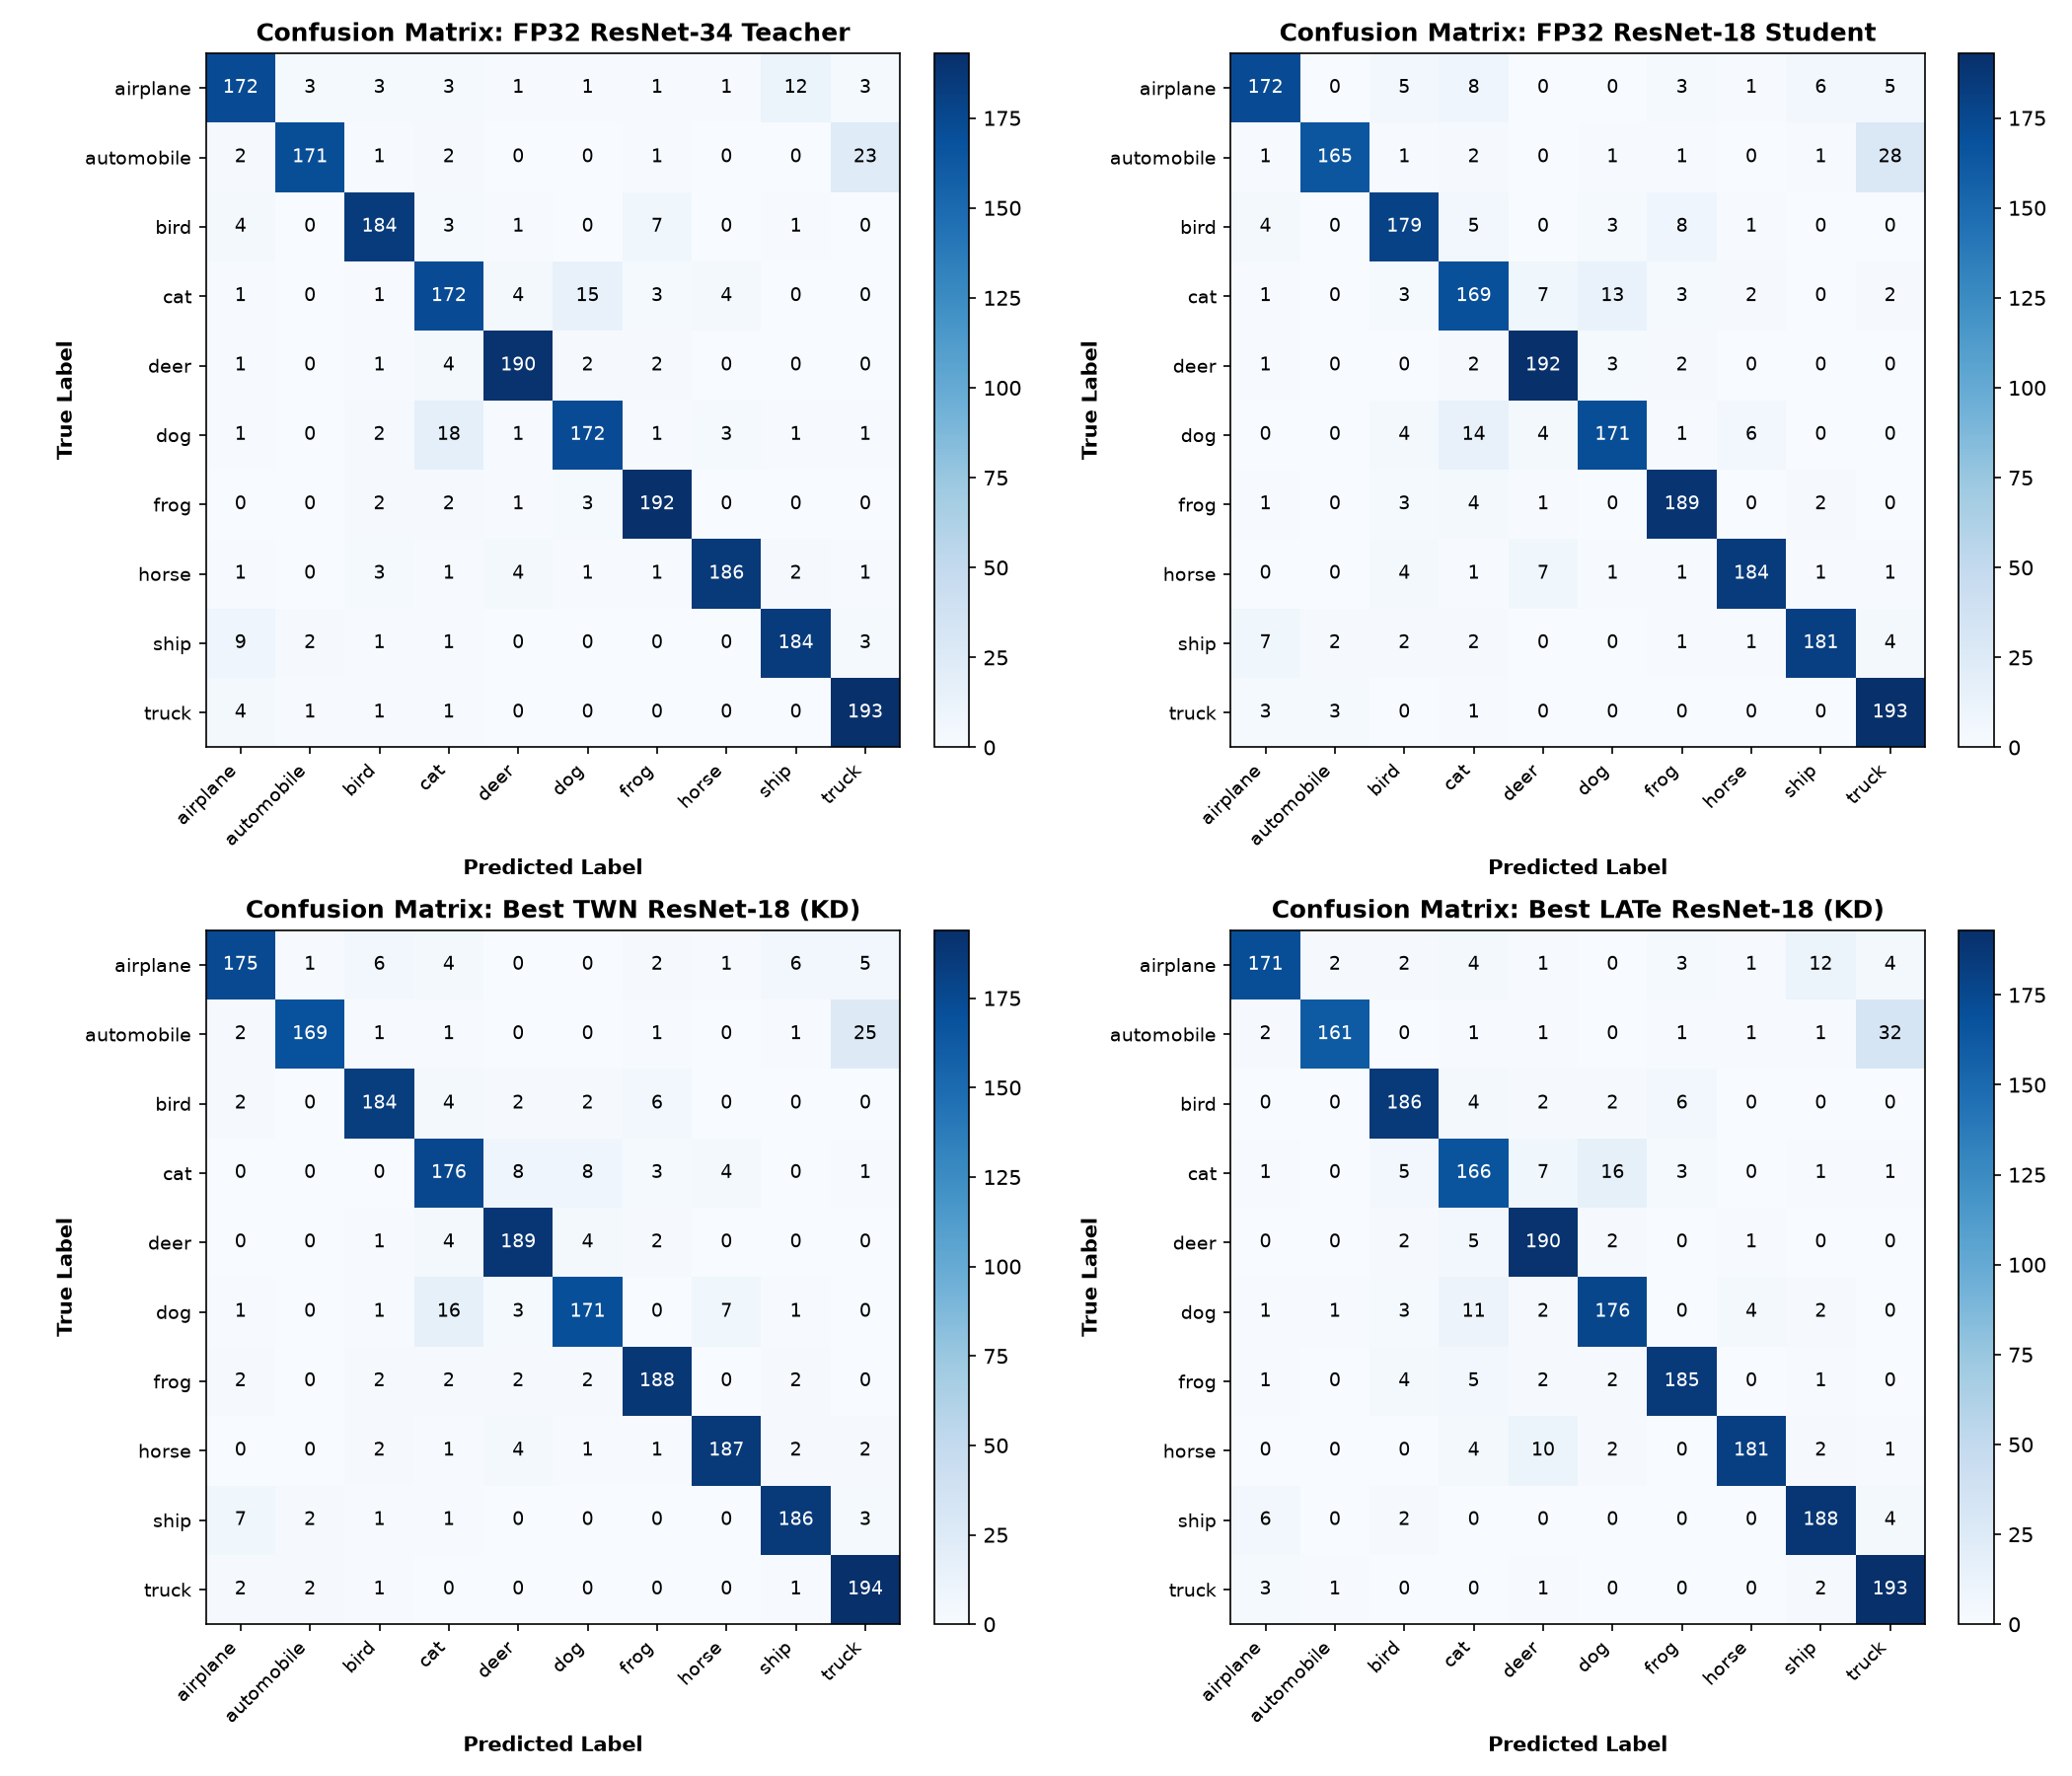
\includegraphics[width=\columnwidth]{unseen_confusion_matrices.png}
\caption{Confusion matrices for the Teacher, Student Base, TWN
Baseline 4, and LATe Baseline 4 on CIFAR-10.1.}
\label{fig:unseen_confusion}
\end{figure}

% ------------------------------------------------------------
% Hardware
% ------------------------------------------------------------

\subsection{Hardware Execution and Compression Potential}

The compression and sparsity results for the main configurations are
summarized in Table~\ref{tab:hardware_compression}.

\begin{table}[H]
\centering
\caption{Storage and sparsity across distinct model configurations.}
\label{tab:hardware_compression}
\scriptsize
\begin{tabular}{@{}lccc@{}}
\toprule
\textbf{Model Configuration} &
\textbf{Sparsity (\%)} &
\textbf{Storage (MB)} &
\textbf{Reduction} \\
\midrule
FP32 Student Base Reference & 0.00 & 42.63 & $1.0\times$ \\
Baseline 1 (TWN Supervised) & 52.00 & 2.72 & $15.7\times$ \\
Baseline 2 (Two-Stage KD+TWN) & 52.00 & 2.72 & $15.7\times$ \\
Baseline 3 (Hard Projection) & 34.91 & 2.72 & $15.7\times$ \\
Baseline 4 (Joint KD + TWN-QAT) & 52.00 & 2.72 & $15.7\times$ \\
Baseline 4 (Full Ternary FNL) & 60.15 & 2.70 & $15.8\times$ \\
Baseline 4 (LATe Loss-Aware) & 66.85 & 2.72 & $15.7\times$ \\
\bottomrule
\end{tabular}
\end{table}

The standard TWN configurations reduce reported model storage from
42.63~MB for the FP32 Student Base to 2.72~MB, corresponding to
approximately a $15.7\times$ reduction. LATe increases overall sparsity
from 52.00\% to 66.85\% under the same reported storage footprint.

The ternary representation also enables multiplication-free weight
operations, where non-zero weights correspond to additions or
subtractions and zero-valued weights can be skipped. Separately, the
theoretical ternary representation requires 2 bits per weight,
providing potential for reduced memory usage and hardware
implementations with fewer general multiplications.

% ------------------------------------------------------------
% Limitations
% ------------------------------------------------------------

\subsection{Experimental Scope and Code Availability}

All reported results correspond to a single deterministic run with
random seed 42. Therefore, the observed differences should be
interpreted as empirical results for this experimental setting rather
than evidence of statistically significant performance differences
across random initializations. The complete implementation, trained
checkpoints, evaluation logs, and visual generation scripts are
available for verification at
\url{https://github.com/vaidhav-adit/Hybrid_KD_and_TWN_QAT}.

% ============================================================
% REFERENCES
% ============================================================

\begin{thebibliography}{00}

\bibitem{he2016}
K.~He, X.~Zhang, S.~Ren, and J.~Sun,
``Deep Residual Learning for Image Recognition,''
in \textit{IEEE Conference on Computer Vision and Pattern Recognition (CVPR)},
pp.~770--778, 2016.

\bibitem{hinton2015}
G.~Hinton, O.~Vinyals, and J.~Dean,
``Distilling the Knowledge in a Neural Network,''
in \textit{NeurIPS Deep Learning and Representation Learning Workshop},
arXiv:1503.02531, 2015.

\bibitem{li2016}
F.~Li, B.~Zhang, and B.~Liu,
``Ternary Weight Networks,''
arXiv:1605.04711, 2016.

\bibitem{zhu2017}
C.~Zhu, S.~Han, H.~Mao, and W.~J.~Dally,
``Trained Ternary Quantization,''
in \textit{International Conference on Learning Representations (ICLR)},
2017.

\bibitem{bengio2013}
Y.~Bengio, N.~L{\'e}onard, and A.~Courville,
``Estimating or Propagating Gradients Through Stochastic Neurons for Conditional Computation,''
arXiv:1308.3432, 2013.

\bibitem{yin2019}
P.~Yin, J.~Lyu, S.~Zhang, S.~Osher, Y.~Ying, and J.~Xin,
``Understanding Straight-Through Estimator in Training Activation Quantized Neural Nets,''
arXiv:1903.05662, 2019.

\bibitem{hou2018lossaware}
L.~Hou and J.~T.~Kwok,
``Loss-Aware Weight Quantization of Deep Networks,''
in \textit{International Conference on Learning Representations (ICLR)},
2018.

\end{thebibliography}

\end{document}